\chapter{Week}
In this week some further testing of the new \ac{DNNDK} version was done. The biggest change here is the added support for the Tensorflow framework. Tensorflow is the most popular neural network training framework right now as figure~\ref{fig:nnframeworks} shows. The x-axis represents the timeline and the y-axis is the percentage of frameworks mentioned in \ac{ML} publications.
\begin{figure}[!htb]
	\centering
		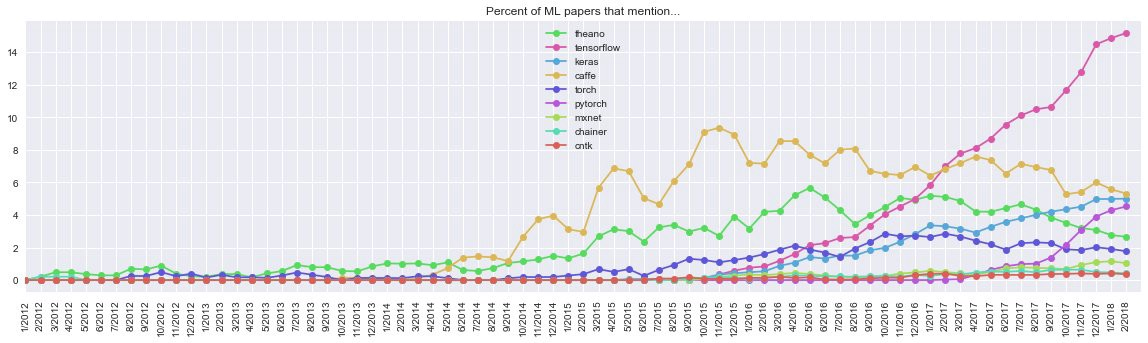
\includegraphics[width=\textwidth]{bilder/nnframeworks.jpg}
		\caption{Neural network framework usage overview \cite{frameworks}}
		\label{fig:nnframeworks}
\end{figure}
Although the output formats of Tensorflow are different than the Caffe output files, the work flow with the \ac{DNNDK} is basically the same as before: take the output of the framework, typically the trained weights and the network structure and feed it to the \ac{DNNDK} tools. Another big change is the separation between each of the tools provided by the \ac{DNNDK} package.
\begin{itemize}
	\item \textbf{\ac{IP} core:} \ac{DPU} \ac{IP} core to be integrated in hardware design
	\item \textbf{\ac{DNNDK} tools:} quantization and compression tools to acquire a binary file encapsulating the trained neural network model
	\item \textbf{\ac{AI} \ac{SDK}:} unified interface providing efficient implementations of common neural network layers as well as common neural networks (see figure~\ref{fig:ai_sdk})
	\begin{figure}[!htb]
		\centering
			\includegraphics[width=\textwidth]{bilder/ai_sdk.png}
			\caption{\ac{AI} \ac{SDK} overview \cite{ai_sdk}}
			\label{fig:ai_sdk}
	\end{figure}
\end{itemize}
The Petalinux documentation was studied as well, especially setting up the device tree correctly. The device tree is a description of the hardware components that are present in a computer system so that the kernel can access these hardware components correctly. Part of this process is automated by the Petalinux tools, however, there are also manual additions that need to be added for the system to work as intended.
After successfully integrating the \ac{DPU} \ac{IP} core into the ZCU 104 evaluation board the implementation of the \ac{DPU} on Enclustra modules was undertaken. Two different modules were chosen from the companies portfolio. One lower end ZYNQ Ultrascale device, the Mars XU3 and a higher end module, the Mercury+ XU1. The main difference concerning \ac{ML} performance is the number of \ac{DSP} blocks on the \acp{FPGA}. The \ac{DPU} can be instantiated in different sizes, the bigger the size the more performance. This is strongly dependent on the number of \ac{DSP} blocks that can be used. A comparison was made which sizes can be synthesized on these two modules. The much bigger Mercury+ XU1 can fit any of the available \ac{DPU} sizes (and has enough room for several instances of the \ac{DPU} \ac{IP} core) whereas the smaller Mars XU3 can only fit small \ac{DPU} sizes.